\section{Introduction}

Recently, diffusion language models (DLMs) have achieved significant progress in
the area of natural language processing ~\cite{nie2025large,bie2025llada2,ye2025dream}.
In traditional autoregressive models (ARs) larguage models, like Llama, and Qwen,
they have the casual attention machenisms, contrastly, DLMs have bi-directional context
understanding and generate the entire context in parallel. Leveraging this
capability, DLMs achieve strong performance in language generation and represent
a promising alternative to AR-based Language Models.

Despite the advantages of parallel decoding, DLMs suffer from high-generation
latency. This bottleneck arises mainly from the bidirectional attention mechanism,
which is central to DLMs. This mechanism computes attention over all query–key token
pairs simultaneously, including both prefill and all generation tokens. As context
length increases, the complexity of this mechanism grows quadratically, leading to
high latency in generation and limiting the efficiency of DLMs in real-world applications.

To balance the generation quality and efficiency, both academia and industry
have proposed various techniques to optimize diffusion strategies and model
architectures. The most adopted approach is called "semi-autoregressive" generation,
which is also known as block diffusion, which sampling applies the origin reverse
process within each block and the autoregressive sampling across blocks. This can make 
KV cache possible during the generation stage, thus reducing the computation cost. \cite{fastdllm}

To address the inference efficiency, sparse attention is an effective method, proposed
in ARs \cite{jiang2024minference}. Some works indentify different attention
scroce (query-key importance) patterns and apply computation masking to reduce
the computation cost. However, directly applying these sparse attention methods
to DLMs is non-trivial due to the unique attention patterns and denoising steps
of DLMs. In DLMs, Some works \cite{wang2025sparsed} try to reuse the initial
attention mask for the following decoding steps. For specific decoding blocks,
it can invert from decoding stage into prefilling stage with the step going, therefore,
the attention score patterns are varing during the whole denoising process. However,
since the attention score patterns are changing during the steps, the initial
attention mask may not be optimal for later steps, leading to harm the model performance.

\xz{ To verify this step-dependent drift, Figure~\ref{fig:cross_step} visualizes how attention score patterns evolve across unmasking steps. 
Figure~\ref{fig:cross_step_heatmap} shows cross-step similarities of the attention-score patterns for several representative query positions. 
Although a few regions maintain relatively high similarity, most steps exhibit clear discrepancies, indicating that attention patterns are not stationary during denoising. 
Figure~\ref{fig:cross_step_curve} further quantifies this phenomenon by plotting the KL divergence between attention patterns of consecutive unmask steps, where sharp spikes reveal abrupt pattern changes at certain steps. 
These observations challenge the implicit assumption behind mask reuse---that the top-$K$ important connections identified at early steps remain top-$K$ for later steps---and motivate us to update the sparse attention mask periodically along the denoising trajectory.}

% Figure 1 illustrates that attention patterns in diffusion LMs are not static along the unmasking trajectory. Figure 1(a) visualizes the cross-step similarity of the attention-score pattern for several representative query positions. While a few steps exhibit high similarity, most steps show noticeable discrepancies, indicating substantial pattern drift as denoising proceeds. Figure 1(b) further quantifies this phenomenon by plotting the KL divergence between attention patterns of consecutive unmask steps. The sharp spikes reveal that the attention distribution can change abruptly at certain steps, rather than evolving smoothly. These observations challenge a common assumption in prior sparse diffusion LMs—namely, that a top-$K$ sparse attention mask computed once at the beginning can be safely reused throughout all subsequent steps. Motivated by this, we propose to periodically refresh the sparse attention mask to better track step-dependent attention dynamics.

In this paper, we introduce a key observation that the attention score patterns share
similarities across different denoising steps in DLMs, but differ significantly
between the prefilling and generation stages. The steps for each block can be divided
into two stages: the prefilling stage and the generation stage. As shown in
Figure~\ref{fig:cross_step} \zz{need cross-step attention map comparasion}, for the block 8, query id from 128 to 144, the attention
score similarities across different steps are different \zz{need data to verify}. 

\begin{figure}[t] % 去掉 *，使其回归单栏
    \centering
    % 第一张子图，宽度设为单栏的 48% 左右
    \begin{subfigure}[b]{0.49\columnwidth}
        \centering
        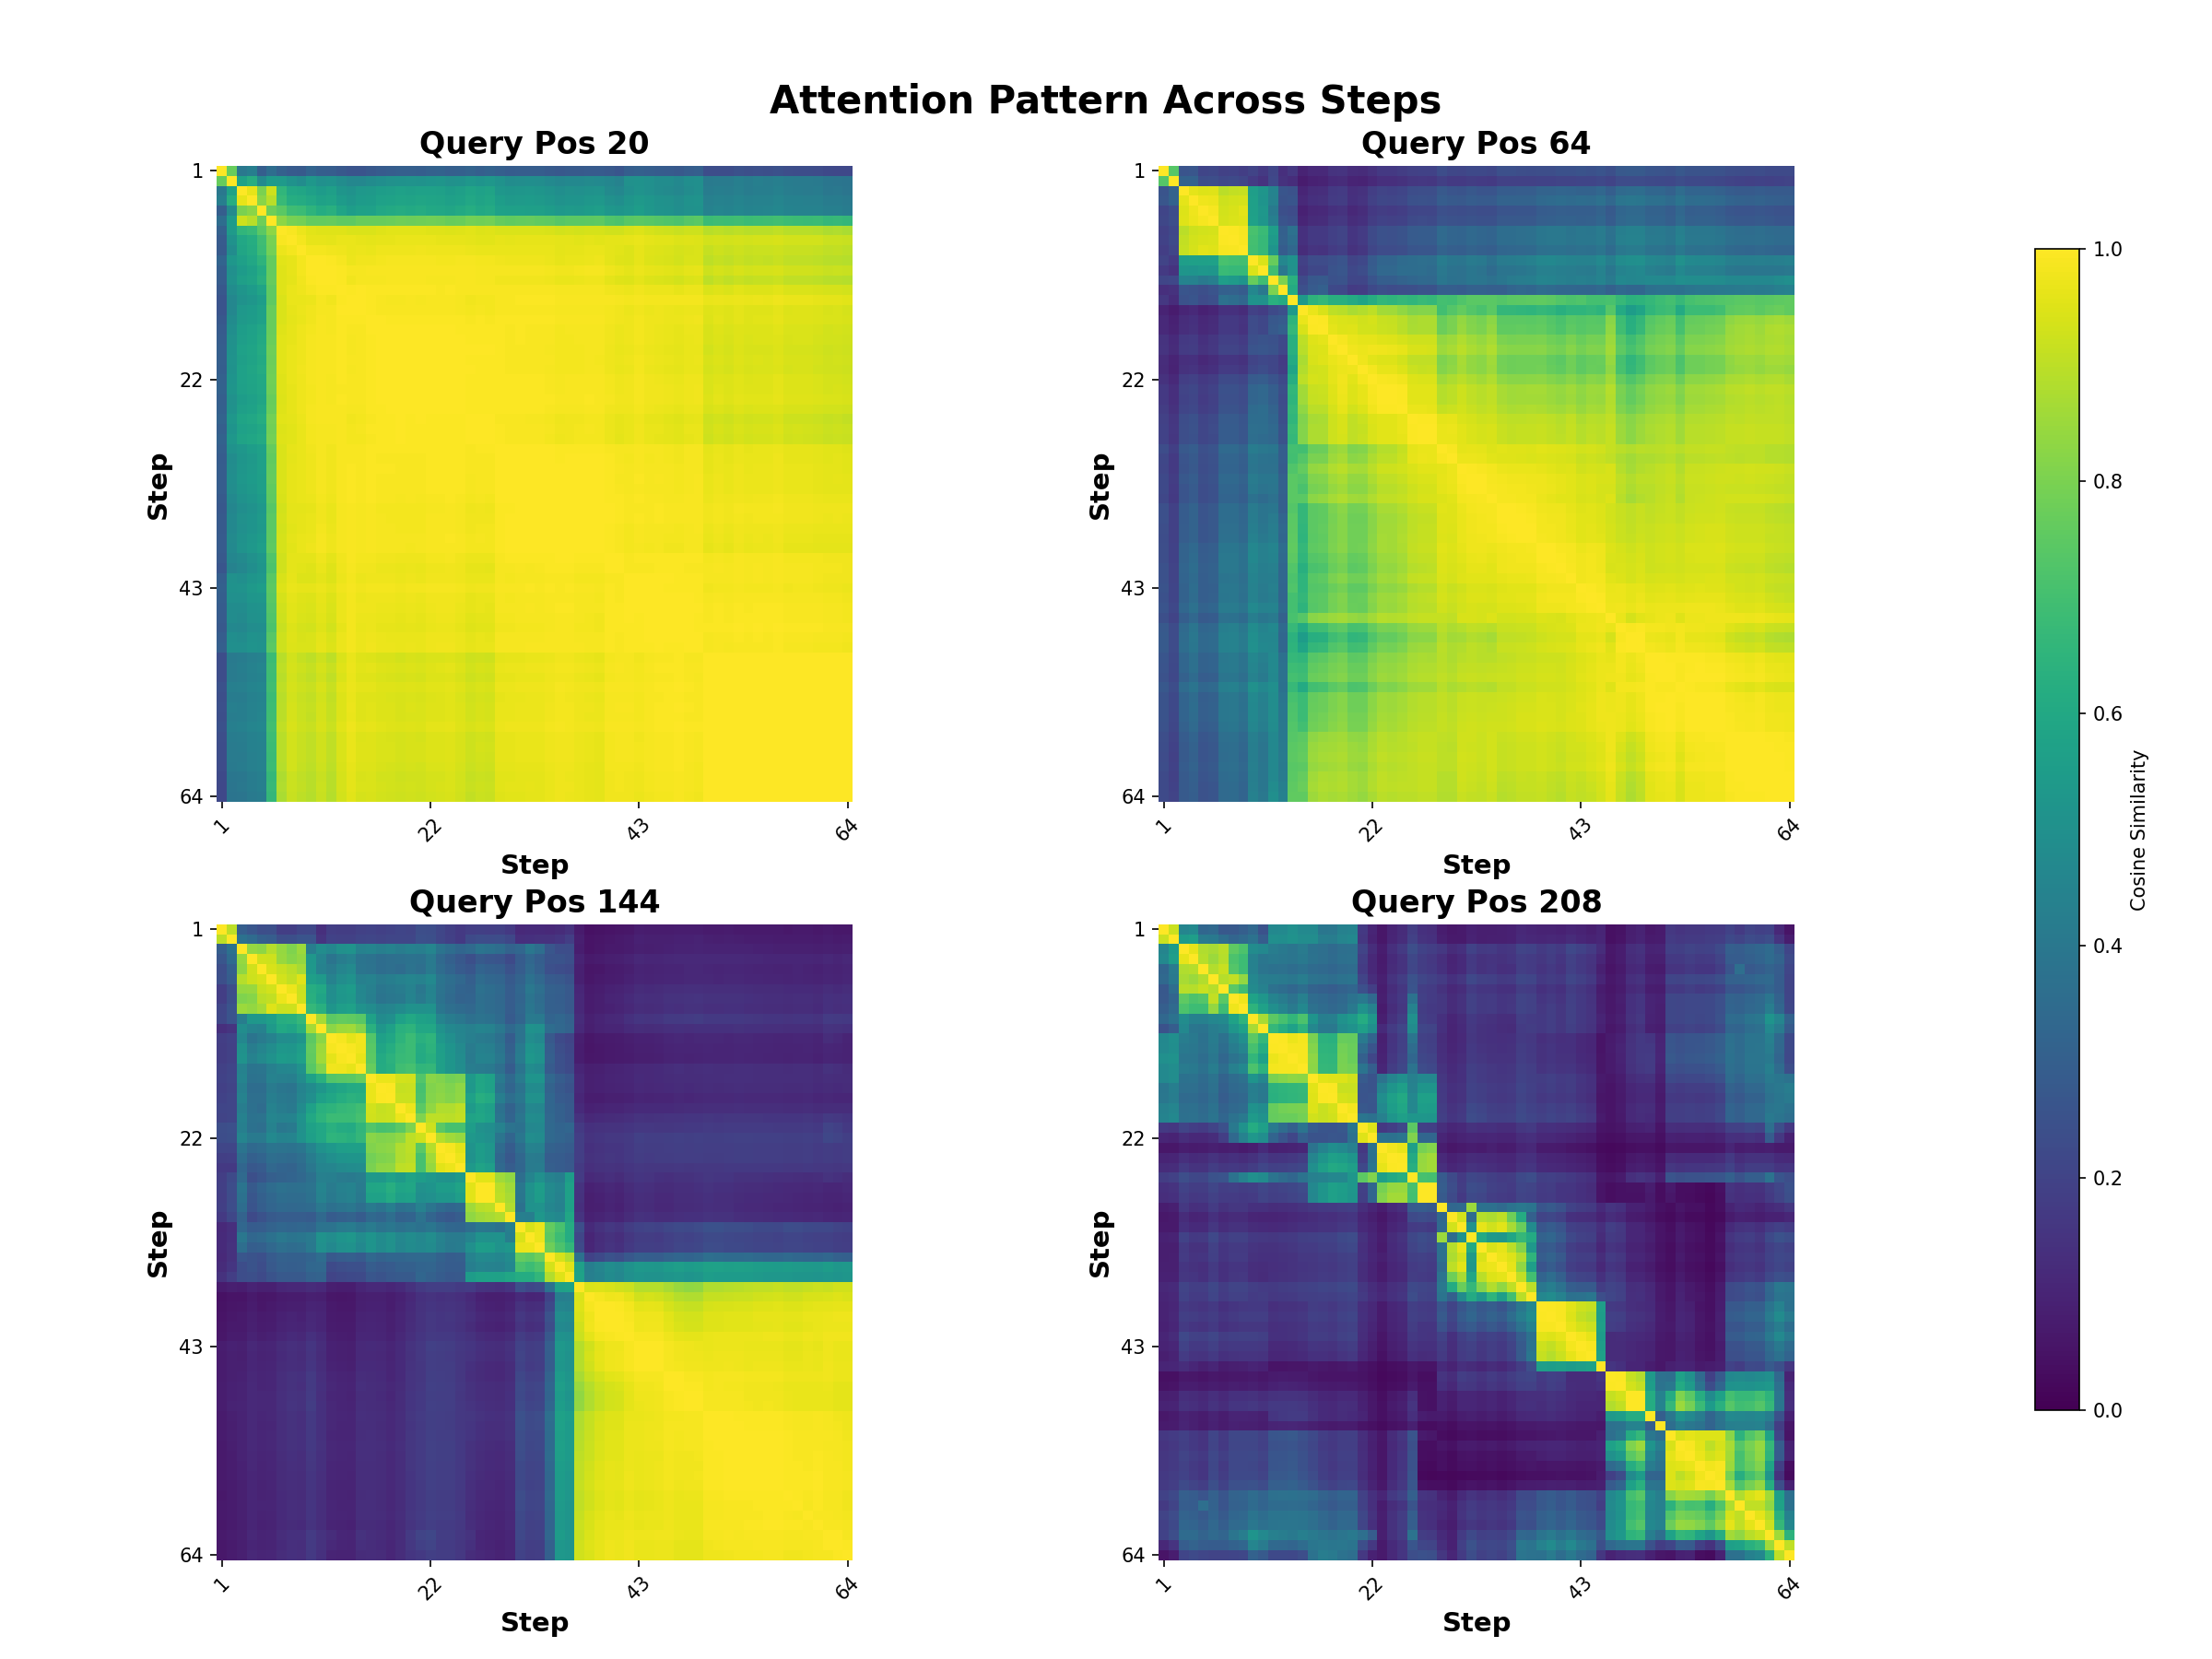
\includegraphics[width=\linewidth]{figures/sample0366_multi_comp_gsm8k_block16_step64_gen256_qpos_20-64-144-208_layer15_head30 (1).png}
        \caption{Step similarities.}
        \label{fig:cross_step_heatmap}
    \end{subfigure}
    \hfill
    % 第二张子图
    \begin{subfigure}[b]{0.49\columnwidth}
        \centering
        
\includegraphics[width=\linewidth]{figures/attention_similarity_curve.png}
        \caption{Step Similarities.}
        \label{fig:cross_step_curve}
    \end{subfigure}
    
    \caption{Comparison of attention pattern visualizations.}
    \label{fig:cross_step}
\end{figure}

\begin{figure}[!t]
    \centering
    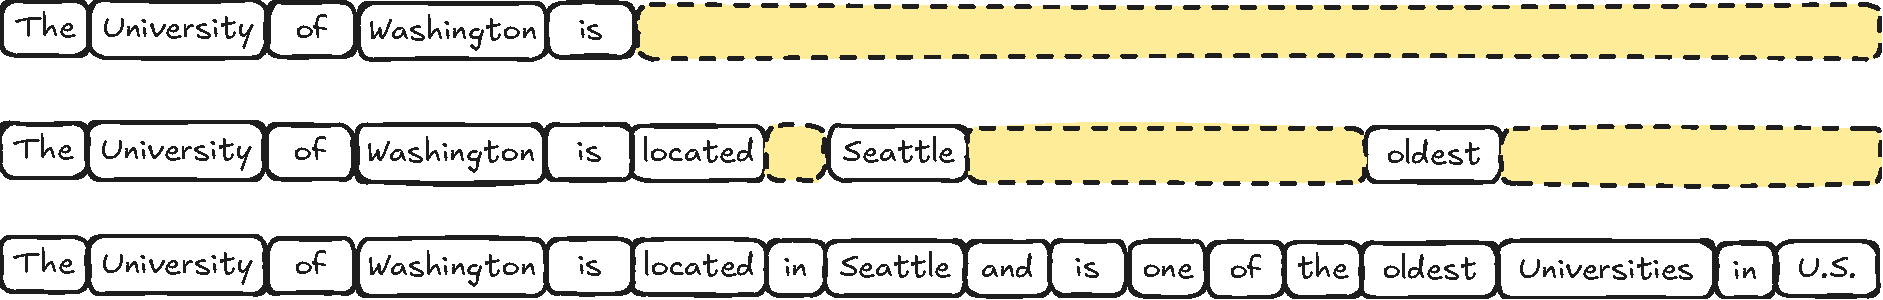
\includegraphics[width=1.0\linewidth]{figures/example.pdf}
    % \vspace{-2em} % 调整图和caption之间的距离
    \caption{Motivation: decoding \& prefilling steps}
    \label{fig:cross_step}
\end{figure}
According to this observation, we propose a novel sparse attention mechanism
tailored for DLMs, which we term Step-aware Sparse Attention (SASA). SASA
dynamically adjusts the attention computation based on the denoising step and
stage (prefilling vs. generation). Besides, we design a global budget
allocation strategy to optimally select the important attention scores to compute across heads,
and design an efficient kernel to implement the sparse attention mechanism, which 
keep the accuracy with significant speedup.

In. summary, our contributions are as follows:
\begin{itemize}
    \item We identify the unique attention score patterns in DLMs across different
    denoising steps and stages, providing insights into the design of efficient
    attention mechanisms for DLMs.
    \item We propose Step-aware Sparse Attention, a novel sparse attention
    mechanism that dynamically adjusts attention computation based on denoising
    steps and stages in DLMs.
    \item We design a global budget allocation strategy and an efficient kernel
    to implement, achieving significant speedup while maintaining generation
    quality.
    \item We conduct extensive experiments on benchmark datasets to validate
    the effectiveness of our proposed method, demonstrating its superiority over
    existing approaches in terms of both efficiency and generation quality.
\end{itemize}

% We argue that DLMs can separate the denoising stages prefilling, and generation stage
% with selective mask updates, and we design an efficient kernle to mask updates
% are across all head global budget.

% In AR models, mask update only occurs in decoding stage

% DLLM model intrinsically has the same attention map compute during the whole decoding
% stages, unlike AR model, each query has its own similarity with others (need to
% revise?)

% In AR, initial token query decide the sparse pattern,